% Short class version (at most 3 pages) of housewives-game.tex.
% Compile: pdflatex housewives-game-short.tex (twice). Check: pdffonts (all Type 1, uni = yes).
% Every number is copied from housewives-game.tex, which housewives-check.py asserts; none is new here.
\documentclass[10pt,a4paper]{article}
\usepackage[utf8]{inputenc}
\usepackage[T1]{fontenc}
\usepackage{lmodern}   % Type 1 vector fonts (replaces PK bitmaps)
\usepackage{cmap}      % ToUnicode CMap -> copyable text and accents
\usepackage[english]{babel}
\usepackage{amsmath,amssymb,mathtools}
\usepackage{textcomp}
\usepackage[a4paper,margin=1.8cm,top=1.6cm,bottom=1.6cm]{geometry}
\usepackage{microtype}
\usepackage{booktabs,array}
\usepackage{enumitem}
\usepackage{xcolor}
\usepackage{tikz}
\usepackage[most]{tcolorbox}
\usepackage{fancyhdr}
\usepackage[hidelinks]{hyperref}

\setlist{topsep=2pt,itemsep=1pt}
\setlength{\parindent}{0pt}
\setlength{\parskip}{4pt}

\pagestyle{fancy}\fancyhf{}
\lhead{\footnotesize Economics of Organizations and Incentives --- MPE Insper}
\rhead{\footnotesize Case: Of housewives and feminists as a game (short version)}
\cfoot{\footnotesize\thepage}
\renewcommand{\headrulewidth}{0.3pt}
\setlength{\headheight}{13pt}

\makeatletter
\renewcommand\section{\@startsection{section}{1}{\z@}{6pt plus 2pt}{2pt}{\normalfont\large\bfseries}}
\makeatother

\definecolor{ans}{RGB}{20,110,70}
\definecolor{src}{RGB}{30,80,150}
\definecolor{warn}{RGB}{190,90,20}
\newcommand{\ours}{\textcolor{warn}{\textbf{[Ours]}}}
\newcommand{\C}{\mathrm{C}}
\newcommand{\Fm}{\mathrm{F}}

\begin{document}

\begin{center}
{\Large\bfseries Of Housewives and Feminists as a Game --- class version}\\[2pt]
{\small Lecture 3 case. Short version of \texttt{Cases/Housewive and feminists/housewives-game.pdf},
where every derivation is worked out. Paper: G\"orges (2021), \emph{Labour Economics} 72, 102044;
``p.~N'' = article page. Amounts in ECU (1 ECU = 1 euro cent). \ours{} marks our analysis, not the paper's.}
\end{center}

\section*{(2) The game}
Real couples (192 subjects) play a one-shot battle of the sexes, simultaneously and without
communication, once with the partner and once with a stranger (pp.~2--4). \textbf{Players:} woman
$W$, man $M$. \textbf{Actions:} Career ($\C$) or Family ($\Fm$); in the Neutral frame they are $A$ and
$B$ and the payoffs are identical. \textbf{Payoffs} (Table 1, p.~3, $\alpha=200$, $\beta=100$): the
Career player against a Family partner gets $200$, the Family player $100$, mis-coordination $0$.

\begin{center}
\begin{tabular}{cc|cc}
 & & \multicolumn{2}{c}{\textbf{Man}}\\
 & & $\C$ & $\Fm$ \\ \hline
\textbf{Woman} & $\C$ & $0,\ 0$ & $\mathbf{200},\ \mathbf{100}$ \\
 & $\Fm$ & $\mathbf{100},\ \mathbf{200}$ & $0,\ 0$ \\
\end{tabular}
\end{center}

\section*{(3) Equilibria}
\textbf{Pure NE:} $(\C,\Fm)$ (Progressive, female-favouring) and $(\Fm,\C)$ (Traditional,
male-favouring); total payoff $300$.

\textbf{Mixed NE (principle of indifference).} Let $q=\Pr(M\text{ plays }\C)$. The woman gets
$u_W(\C,q)=200(1-q)$ and $u_W(\Fm,q)=100\,q$; she is indifferent iff $q=\tfrac{200}{300}=\tfrac23$, and
prefers $\C$ iff $q<\tfrac23$. By symmetry $p=\Pr(W\text{ plays }\C)=\tfrac23$. Each player's mix is
pinned down by the \emph{other's} payoffs.

\begin{tcolorbox}[colback=ans!5,colframe=ans,boxrule=0.6pt,left=5pt,right=5pt,top=3pt,bottom=3pt]
\textbf{Mixed NE:} $\Pr(\C)=\tfrac{\alpha}{\alpha+\beta}=\tfrac23$ each; $u=\tfrac{\alpha\beta}{\alpha+\beta}=\tfrac{200}{3}\approx66.7$
(p.~3). Outcomes: Progressive $\tfrac29$, Traditional $\tfrac29$, both-Career $\tfrac49$, both-Family
$\tfrac19$, so coordination is $\tfrac49\approx44.4\%$ (``just below 45\%'', p.~3). Total payoff
$2\times\tfrac{200}{3}\approx133.3$, against $300$ in a pure NE: the mixed NE is equal but
inefficient, the pure NE efficient but unequal ($200$ against $100$).
\end{tcolorbox}

\section*{(4) Focal points}
Schelling (1960): a salient label can select an equilibrium without changing payoffs, by making one
outcome the common expectation. The paper's hypothesis (p.~3): the Career/Family label makes the
Traditional equilibrium focal, so it is reached more often, ``improving efficiency at the cost of
increased inequality to the disadvantage of women''. In game terms the label shifts beliefs: a woman
who expects the man to play $\C$ with probability above $\tfrac23$ best-responds with $\Fm$. This is
the efficiency--equality trade-off: total payoff moves toward $300$, but the man gets $200$ and the
woman $100$.

\section*{(5) Theory against the data}
\begin{center}\small
\begin{tabular}{lcccc}
\toprule
Career rate (Table 4 col.~1, p.~8) & Men Neutral & Women Neutral & Men Norm & Women Norm \\
\midrule
Observed & $0.536$ & $0.563$ & $0.625$ & $0.250$ \\
\bottomrule
\end{tabular}
\end{center}
\textbf{Outcomes} (Table 3 col.~2, p.~6): Norm versus Neutral changes Progressive by $-0.171$,
Traditional by $+0.255$, non-coordination by $-0.085$. \textbf{Earnings} (Table C1, p.~15): Norm men
$112.50$, women $75.00$ (women earn $\tfrac23$, ``67\% of men'', p.~7); Neutral men $80.36$, women $83.04$.

\ours{} \textbf{Best responses against the real rates.} A woman in Norm facing men's $0.625$: $\C$ pays
$0.375\times200=75$, $\Fm$ pays $0.625\times100=62.5$, so Career was her best response, yet only $25\%$
chose it. A man facing women's $0.25$: $\C$ pays $150$, $\Fm$ pays $25$. Women's beliefs about men
overshoot the true rates (fn.~27, p.~9); with a belief above $\tfrac23$, $\Fm$ is the woman's best response.

\ours{} \textbf{Independence benchmark} (\emph{ours, not the paper's}): with the observed rates and independent
choices, Neutral gives Progressive $0.261$, Traditional $0.234$, coordination $0.495$; Norm gives
$0.094$, $0.469$ and $0.5625$. Expected Norm earnings: men $103.1$, women $65.6$, below the observed
$112.50$ and $75.00$, so pairs coordinate more than independent play implies. Total earnings per
couple rise from $163.4$ to $187.5$ with the Norm label, but men gain $32.14$ and women lose $8.04$.
\textbf{Own-payoff puzzle} (ours): an identity utility $n$ for women choosing Family would move
the \emph{men's} mix, $\tfrac{200-n}{300}$, not the women's; the data move the women, which points to
equilibrium selection (a focal point) rather than a payoff shift.

\section*{(8) Dynamics: the sequential BoS}
If the woman moves first and the man observes her move, backward induction gives: after $\C$ he plays
$\Fm$ ($100>0$); after $\Fm$ he plays $\C$ ($200>0$); she compares $\C\to200$ with $\Fm\to100$ and plays $\C$.

\begin{center}
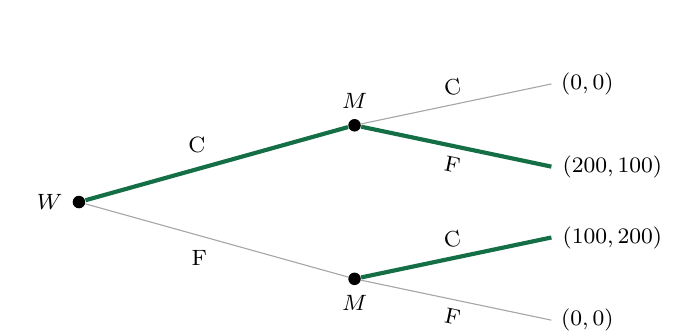
\begin{tikzpicture}[x=1.0cm,y=0.75cm,every node/.style={font=\footnotesize},
  dec/.style={circle,fill,inner sep=1.6pt},
  spe/.style={draw=ans,line width=1.5pt},e/.style={draw=gray!70}]
  \node[dec,label=left:$W$] (r) at (0,0) {};
  \node[dec,label=above:$M$] (a) at (3.5,1.3) {};
  \node[dec,label=below:$M$] (b) at (3.5,-1.3) {};
  \draw[spe] (r) -- node[above left]{$\C$} (a);
  \draw[e] (r) -- node[below left]{$\Fm$} (b);
  \draw[e] (a) -- node[above,sloped]{$\C$} (6,2) node[right]{$(0,0)$};
  \draw[spe] (a) -- node[below,sloped]{$\Fm$} (6,0.6) node[right]{$(200,100)$};
  \draw[spe] (b) -- node[above,sloped]{$\C$} (6,-0.6) node[right]{$(100,200)$};
  \draw[e] (b) -- node[below,sloped]{$\Fm$} (6,-2) node[right]{$(0,0)$};
\end{tikzpicture}
\end{center}
\textbf{SPE:} $W$ plays $\C$; $M$ plays $\Fm$ after $\C$ and $\C$ after $\Fm$; payoffs $(200,100)$. The
first mover gets $200$, against $\tfrac{200}{3}\approx66.7$ in the mixed NE, a gain of
$\tfrac{400}{3}\approx133.3$. There is also a Nash equilibrium that is not subgame perfect,
$(\Fm;\ \C,\C)$ with payoffs $(100,200)$, resting on the threat ``I play Career whatever you do'':
after $\C$ the man would get $0$ by carrying it out and $100$ from $\Fm$, so it is not credible.
\textbf{Commitment} is valuable: whoever commits first (job offer, first child) is the one the
other must best-respond to. \textbf{Path dependence} (fn.~12, p.~4): today's specialisation raises
the payoff of repeating it tomorrow.
\ours{} \textbf{Lecture 5 preview:} alternating $(\C,\Fm),(\Fm,\C),\dots$ gives $150$ per period each
against $\tfrac{200}{3}$ for repeating the mixed NE.

\begin{tcolorbox}[colback=src!4,colframe=src,boxrule=0.5pt,left=5pt,right=5pt,top=3pt,bottom=3pt,
  title={Takeaway}]
\begin{itemize}[leftmargin=1.2em]
  \item The one-shot BoS has two efficient but unequal pure equilibria and an inefficient mixed one
    ($\Pr(\C)=\tfrac23$, payoff $\tfrac{200}{3}$, coordination $\tfrac49$); theory alone does not say which is played.
  \item The Norm label acts as a focal point: women's Career rate falls from $0.563$ to $0.250$,
    the Traditional outcome rises by $0.255$ and women earn $\tfrac23$ of men's earnings, with no change in payoffs.
  \item Moving first is worth $133.3$ ECU; the credible commitment, not the threat, decides who
    specialises in Career.
\end{itemize}
\end{tcolorbox}

\end{document}
